\documentclass[Measurements]{subfiles}
\begin{document}
\section{Measurements}
\label{sec:Measurements}

\subsection{Expermimental setup}
\begin{figure}[h]
\caption{Experimental setup}
\centering
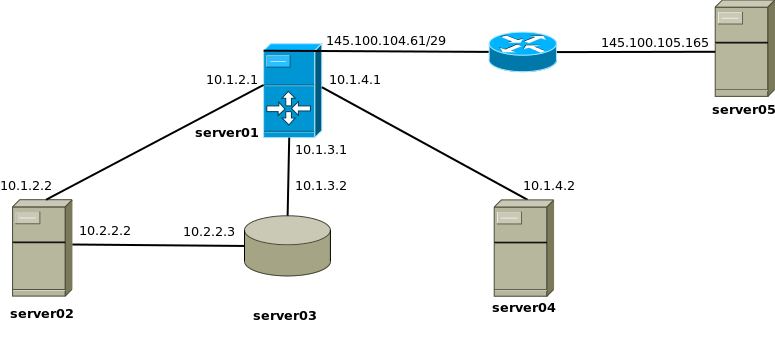
\includegraphics[scale=0.4] {images/infrastructure.png}
\label{fig:Experimental setup}
\end{figure}

As there is no standard set of rules for performance testing web servers, the described definition aims at being, what in medicine is called, a gold standard test~\cite{wacholder1993validation}.
In order to The following things are vital to performance testing:

\begin{description} 
 \item[server-side] text 
 \item[client-side] text
\end{description}


\end{document}

